\documentclass[]{book}
\usepackage{lmodern}
\usepackage{amssymb,amsmath}
\usepackage{ifxetex,ifluatex}
\usepackage{fixltx2e} % provides \textsubscript
\ifnum 0\ifxetex 1\fi\ifluatex 1\fi=0 % if pdftex
  \usepackage[T1]{fontenc}
  \usepackage[utf8]{inputenc}
\else % if luatex or xelatex
  \ifxetex
    \usepackage{mathspec}
  \else
    \usepackage{fontspec}
  \fi
  \defaultfontfeatures{Ligatures=TeX,Scale=MatchLowercase}
\fi
% use upquote if available, for straight quotes in verbatim environments
\IfFileExists{upquote.sty}{\usepackage{upquote}}{}
% use microtype if available
\IfFileExists{microtype.sty}{%
\usepackage{microtype}
\UseMicrotypeSet[protrusion]{basicmath} % disable protrusion for tt fonts
}{}
\usepackage{hyperref}
\hypersetup{unicode=true,
            pdftitle={Impact Malaria Data Hub Specifications},
            pdfauthor={Isaiah Nyabuto, Cristina Lussiana},
            pdfborder={0 0 0},
            breaklinks=true}
\urlstyle{same}  % don't use monospace font for urls
\usepackage{natbib}
\bibliographystyle{apalike}
\usepackage{longtable,booktabs}
\usepackage{graphicx,grffile}
\makeatletter
\def\maxwidth{\ifdim\Gin@nat@width>\linewidth\linewidth\else\Gin@nat@width\fi}
\def\maxheight{\ifdim\Gin@nat@height>\textheight\textheight\else\Gin@nat@height\fi}
\makeatother
% Scale images if necessary, so that they will not overflow the page
% margins by default, and it is still possible to overwrite the defaults
% using explicit options in \includegraphics[width, height, ...]{}
\setkeys{Gin}{width=\maxwidth,height=\maxheight,keepaspectratio}
\IfFileExists{parskip.sty}{%
\usepackage{parskip}
}{% else
\setlength{\parindent}{0pt}
\setlength{\parskip}{6pt plus 2pt minus 1pt}
}
\setlength{\emergencystretch}{3em}  % prevent overfull lines
\providecommand{\tightlist}{%
  \setlength{\itemsep}{0pt}\setlength{\parskip}{0pt}}
\setcounter{secnumdepth}{5}
% Redefines (sub)paragraphs to behave more like sections
\ifx\paragraph\undefined\else
\let\oldparagraph\paragraph
\renewcommand{\paragraph}[1]{\oldparagraph{#1}\mbox{}}
\fi
\ifx\subparagraph\undefined\else
\let\oldsubparagraph\subparagraph
\renewcommand{\subparagraph}[1]{\oldsubparagraph{#1}\mbox{}}
\fi

%%% Use protect on footnotes to avoid problems with footnotes in titles
\let\rmarkdownfootnote\footnote%
\def\footnote{\protect\rmarkdownfootnote}

%%% Change title format to be more compact
\usepackage{titling}

% Create subtitle command for use in maketitle
\providecommand{\subtitle}[1]{
  \posttitle{
    \begin{center}\large#1\end{center}
    }
}

\setlength{\droptitle}{-2em}

  \title{Impact Malaria Data Hub Specifications}
    \pretitle{\vspace{\droptitle}\centering\huge}
  \posttitle{\par}
    \author{Isaiah Nyabuto, Cristina Lussiana}
    \preauthor{\centering\large\emph}
  \postauthor{\par}
      \predate{\centering\large\emph}
  \postdate{\par}
    \date{2019-11-18}

\usepackage{booktabs}
\usepackage{amsthm}
\makeatletter
\def\thm@space@setup{%
  \thm@preskip=8pt plus 2pt minus 4pt
  \thm@postskip=\thm@preskip
}
\makeatother

\begin{document}
\maketitle

{
\setcounter{tocdepth}{1}
\tableofcontents
}
\hypertarget{welcome}{%
\chapter*{Welcome}\label{welcome}}
\addcontentsline{toc}{chapter}{Welcome}

This is a technical guide for the IM Data Hub, \textbf{a work currently in progress by BAO systems intended for official release in \href{imdatahub.org}{production} by }\_\_\_\_

\href{imdatahub.org}{IM Data Hub} is a warehouse for Impact Malaria indicator data. It houses all the IM indicator data for project performance monitoring and use. It is primarily designed with data users in mind, and it comes with several tools specifically designed to promote the use of IM data.

To date, IM Data Hub is active in 11 countries in Africa, and it collects a tremendous amount of data in the following tracks;

\begin{enumerate}
\def\labelenumi{\arabic{enumi}.}
\tightlist
\item
  case management
\item
  Malaria in Pregnancy
\item
  Seasonal Malaria Chemoprevention
\item
  Global Technical Leadership.
\end{enumerate}

It is used by multiple partners at different levels, from donors (PMI), Implementers (PSI, Jhpiego, UCSF, e.t.c), and government ministries of health in tracking country performance.

\hypertarget{preface}{%
\chapter*{Preface}\label{preface}}
\addcontentsline{toc}{chapter}{Preface}

\hypertarget{what-is-this-guide}{%
\section{What is this guide?}\label{what-is-this-guide}}

This guide provides information about the technical specifications of the Impact Malaria (IM) Data Hub. It's meant to guide the development, testing \& customization of the database for IM indicator data.

\hypertarget{who-should-read-this-guide}{%
\section{Who should read this guide?}\label{who-should-read-this-guide}}

This guide is aimed at two main audiences.

\begin{itemize}
\tightlist
\item
  System Administrators who are involved in the administration or the daily operation of IM Data Hub.
\item
  Project teams \& M\&E staff interested to learn more about the IM Data Hub. You will find this helpful in understanding the overall system set up and how different components work together in the system.
\end{itemize}

\hypertarget{what-is-covered.}{%
\section{What is covered.}\label{what-is-covered.}}

The guide is divided into seven chapters.

\begin{enumerate}
\def\labelenumi{\arabic{enumi}.}
\tightlist
\item
  Introduction - offers some background information and how to quickly get started on IM Data Hub.
\item
  Components - describes the IM Data Hub main components and how they are set up.
\item
  Data Specification - `builds on the main components description and talks about the IM indicators and data reporting.
\item
  Metadata Specifications - dives into the data specification and the system components and talks about what lies at the bottom, the metadata.
\item
  Customization \& Troubleshooting - Provides guidance on customization, testing and troubleshooting the IM Data Hub.
\item
  Security and Access Model - Explains the security mechanisms and access model.
\item
  Appendix - Lists down worksheets and some other the materials used in the IM Data Hub.
\end{enumerate}

\hypertarget{conventions}{%
\section{Conventions}\label{conventions}}

This guide follows the following document conventions.

\begin{longtable}[]{@{}ll@{}}
\toprule
Abbreviation & In Full\tabularnewline
\midrule
\endhead
CR & Case Reporting\tabularnewline
IM & Impact Malaria\tabularnewline
SS & Supportive Supervision\tabularnewline
TR & Training\tabularnewline
TL & Technical Leadership\tabularnewline
SMC & Seasonal Malaria Chemoprophylaxis\tabularnewline
DX & Diagnosis\tabularnewline
TX & Treatment\tabularnewline
MIP & Malaria In Pregnancy\tabularnewline
CS & Country Specific\tabularnewline
RE & Reporting\tabularnewline
PMP & Performance Management Plan\tabularnewline
\bottomrule
\end{longtable}

\hypertarget{data-sets}{%
\subsection{Data Sets}\label{data-sets}}

Data set: {[}\texttt{country\ ISO\ code}{]} {[}\texttt{program}{]}:

Examples;

\begin{itemize}
\tightlist
\item
  GH Supportive Supervision
\item
  CD Case Reporting \textbar{}Data set: {[}country ISO code{]} {[}Data entry form name{]}
\end{itemize}

\hypertarget{data-elements}{%
\subsection{Data Elements}\label{data-elements}}

DEs: {[}\texttt{country\ ISO\ code}{]} {[}\texttt{program\ abbreviation}{]} - {[}\texttt{section\ abbreviation}{]} {[}\texttt{DE\ Form\ name}{]}:

Examples;

\begin{itemize}
\tightlist
\item
  GH CR - DX Cases confirmed
\item
  CD TL - DX Does this province have national malaria diagnostic supervision tools that adhere to global standards?
\end{itemize}

\hypertarget{indicators}{%
\subsection{Indicators}\label{indicators}}

Indicators: {[}\texttt{country\ ISO\ code}{]} {[}\texttt{PMP}{]} - {[}\texttt{section\ abbreviation}{]} {[}\texttt{Indicator\ name}{]}:

Example;

CD PMP - DX Percentage of health workers demonstrating competence in malaria microscopy

\hypertarget{acknowledgement}{%
\section{Acknowledgement}\label{acknowledgement}}

\hypertarget{intro}{%
\chapter{Introduction}\label{intro}}

\hypertarget{background}{%
\section{Background}\label{background}}

Impact Maria (IM) Data Hub is a web-based project monitoring system used to collect, analyze, and report indicator data for Impact Malaria Project. IM is a five-year project by the US President's Malaria Initiative (PMI) global service to reduce malaria mortality and morbidity.

The BAO system implements it in an ST-3 plan that began on Nov 27th, 2018.

The system hosts all the IM data. Multiple partners use it at different levels from donors (PMI), implementers (PSI, Jhpiego, UCSF,.e.tc), and government ministries of health (MOH) to track project progress and country performance.

It's active in 11 countries, and collects a tremendous amount of data on;

\begin{enumerate}
\def\labelenumi{\arabic{enumi}.}
\tightlist
\item
  Case Management
\item
  Malaria in pregnancy
\item
  Seasonal Malaria Chemoprevention
\item
  Global Technical Leadership.
\end{enumerate}

IM Data Hub is compatible with HNQIS version 4.

\hypertarget{purpose}{%
\subsection{Purpose}\label{purpose}}

IM Data Hub was developed;

\begin{enumerate}
\def\labelenumi{\arabic{enumi}.}
\tightlist
\item
  To monitor IM indicator data.
\item
  Provide access to IM indicator data at the country and global level.
\item
  Enable central/global level data management
\item
  Track project progress and country performance
\item
  Promote data use for decision making.
\end{enumerate}

\hypertarget{servers}{%
\subsection{Servers}\label{servers}}

IM Data Hub is available at the following instances;

\begin{enumerate}
\def\labelenumi{\arabic{enumi}.}
\tightlist
\item
  Development instance: Where all the developments and testing takes place. It's accessible at \url{https://im-dev.psi-mis.org/} (version 2.30 as of Jan 9, 2019): Analytics run at midnight and 12:00 UTC (EAT -3h)
\item
  Production instance: Ready for use. Accessible at impactmalaria-mis.org (Version 2.30, not ready as of Aug 30, 2019):
\end{enumerate}

\hypertarget{getting-started}{%
\section{Getting Started}\label{getting-started}}

The easiest way to get started to IM Data Hub is to log in at the test server at \url{https://im-dev.psi-mis.org/} with the following credentials.

\texttt{Username\ :}\textbf{\texttt{demoUser}} \texttt{and\ Password\ :} \textbf{\texttt{Temp1234!}}

The landing page!

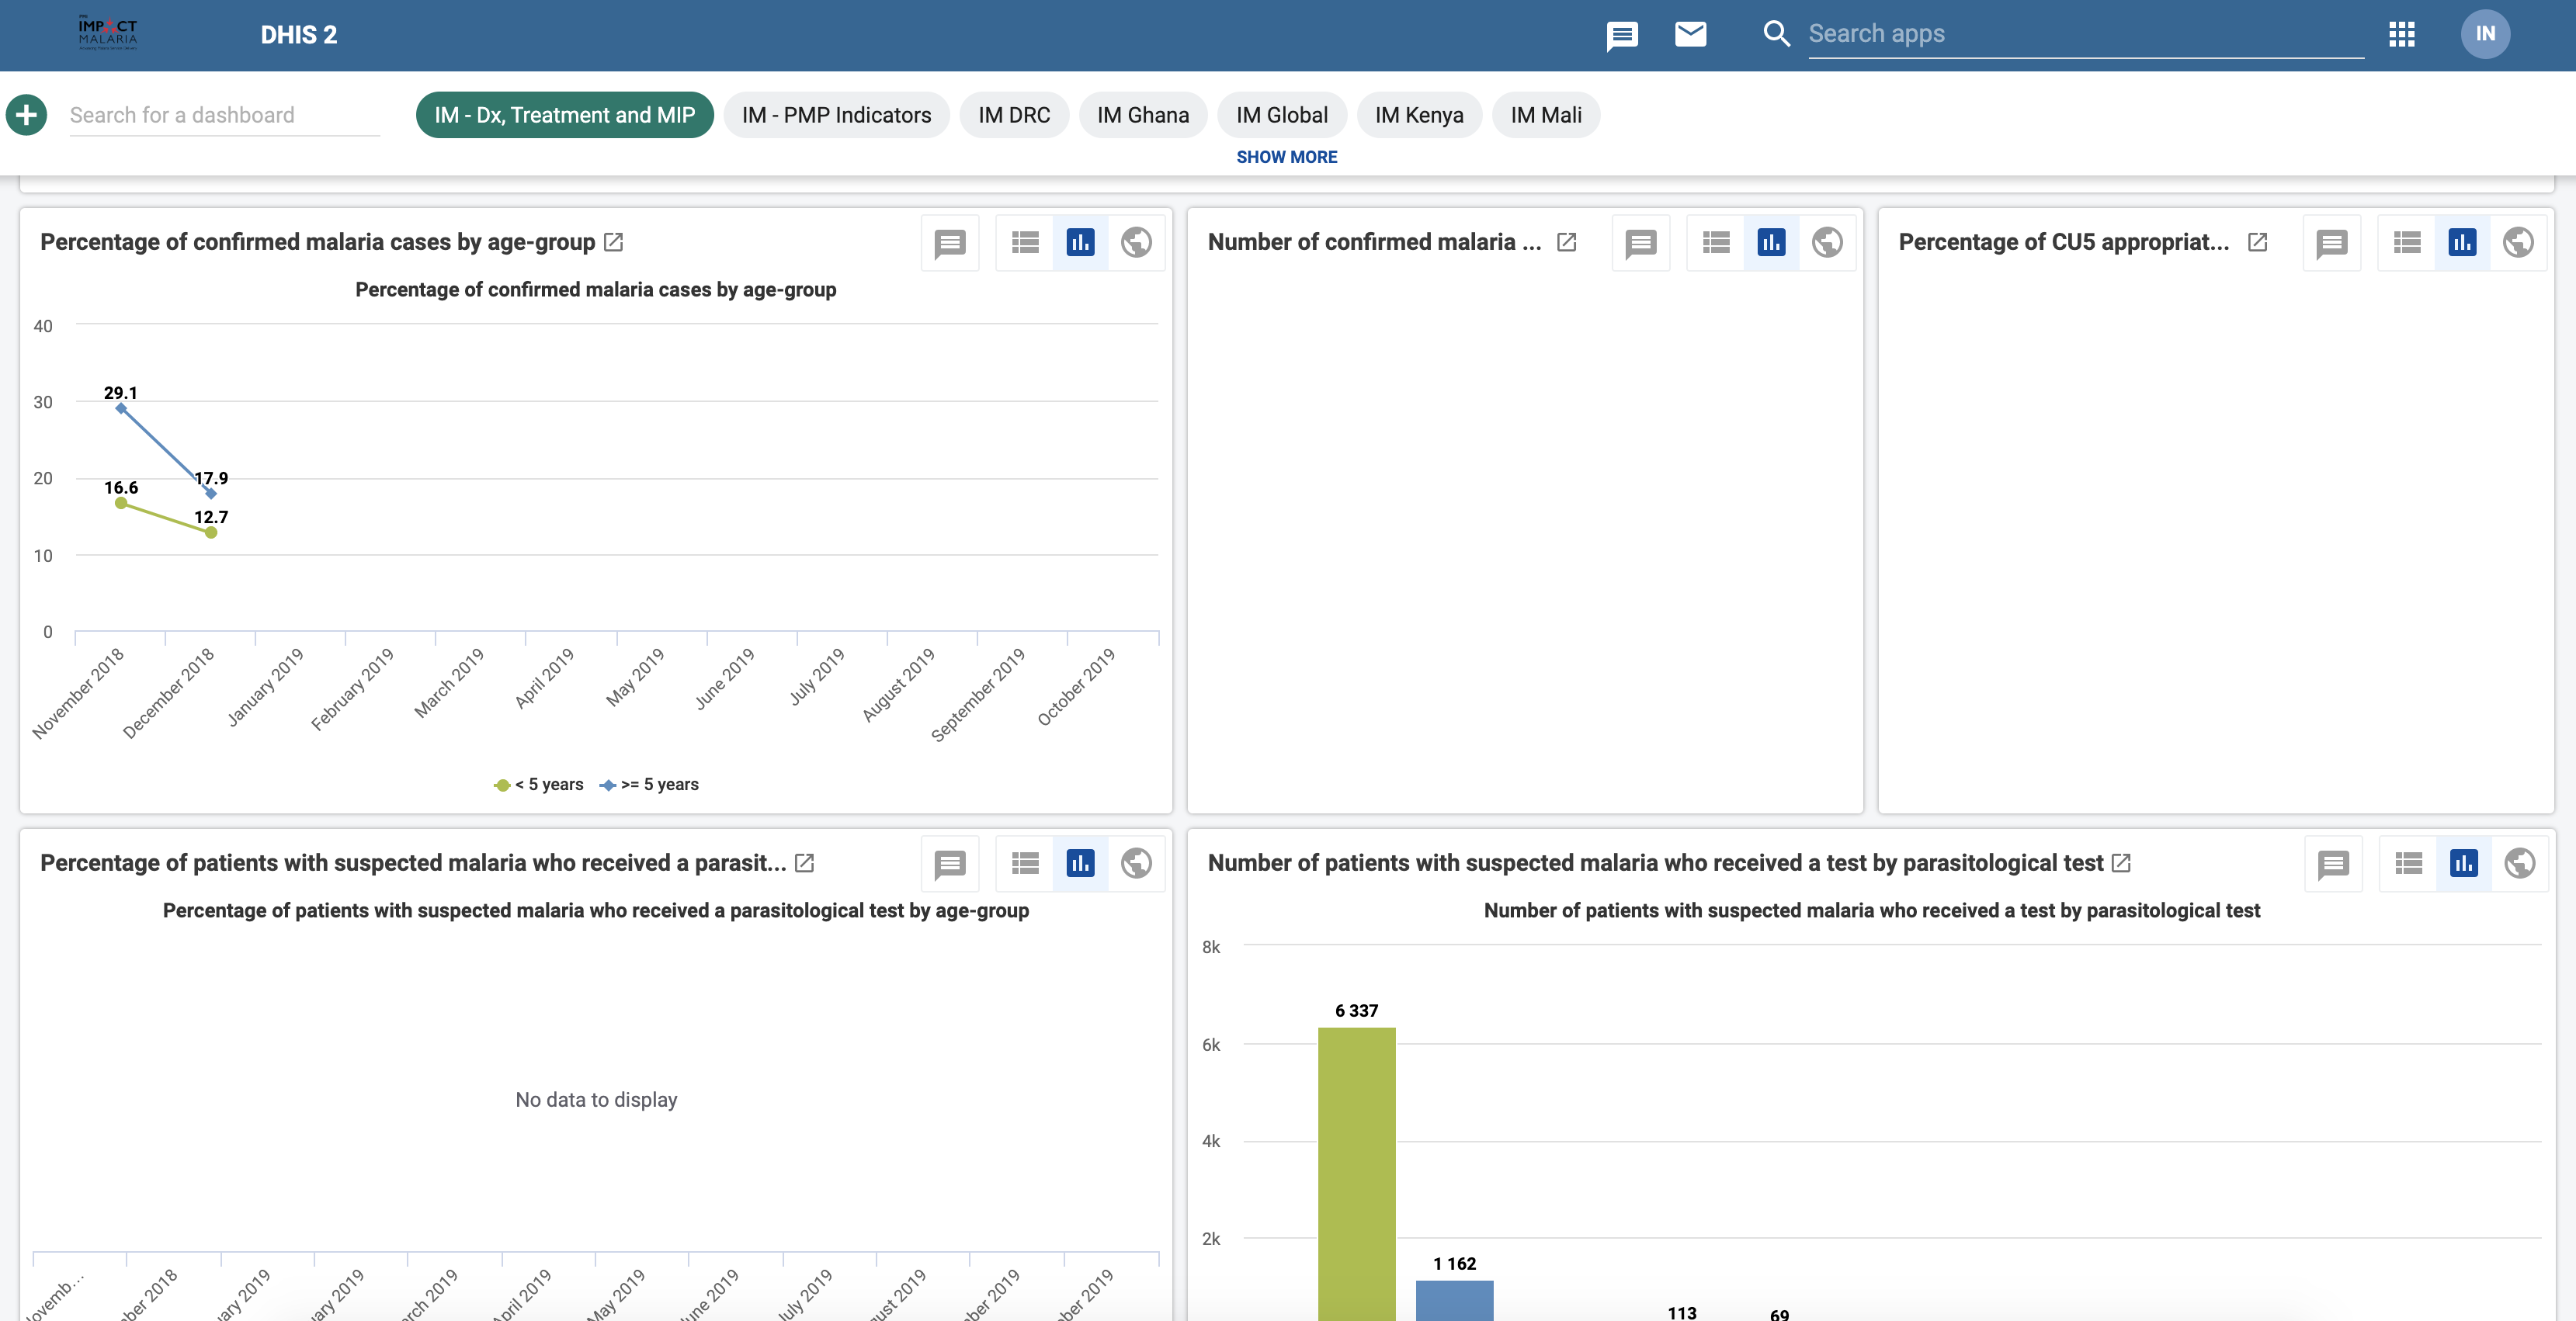
\includegraphics[width=46.08in]{./images/landing-page}

Countries doing data entry or testings can log in with the following credentials based on their country ISO codes.

\begin{longtable}[]{@{}ll@{}}
\toprule
Country & username ; password\tabularnewline
\midrule
\endhead
Congo & \texttt{CDdemo};\texttt{Temp1234!}\tabularnewline
Cameroon & \texttt{CMdemo};\texttt{Temp1234!}\tabularnewline
Ghana & \texttt{GHdemo};\texttt{Temp1234!}\tabularnewline
Kenya & \texttt{KEdemo};\texttt{Temp1234!}\tabularnewline
Mali & \texttt{MLdemo};\texttt{Temp1234!}\tabularnewline
Niger & \texttt{NEdemo};\texttt{Temp1234!}\tabularnewline
\bottomrule
\end{longtable}

\hypertarget{understanding-im-data-hub}{%
\chapter{Understanding IM Data Hub}\label{understanding-im-data-hub}}

\hypertarget{introduction}{%
\section{Introduction}\label{introduction}}

Now that you're already started and you've got some essential background about IM Data Hub, we are going to explore the details/components that form IM Data Hub.

As we saw in the previous chapter, IM Data Hub is not just a database; it's a project monitoring system. It's divided into components; whose primary goal is to monitor IM indicator data for action.

We'll dive deeper into the components and understand how they are set up in the Hub.

Understanding IM Data Hub components will allow you to report, analyse, and monitor IM indicators more effectively.

I'll start by showing the you reporting component, IM Data Hub uses data sets to collect indicator data. We will discuss them briefly in the next section. We will then walk through the data mining piece, and how the different outputs are pulled together on a dashboard for the project use. We'll wind up by exploring the data quality component and how the IM indicator data pass through the quality checks.

\hypertarget{reporting-component}{%
\section{Reporting Component}\label{reporting-component}}

Reporting is organized through the use of data sets. A data set is simply a list of data elements that are grouped for data collection. We'll talk more about data elements in the next chapter.

A data set has a reporting period and an organization unit. The reporting period specifies how the data is reported, i.e., monthly, or quarterly, while the organization unit determines the location ``where'' the information is collected.

IM Data Hub has two main types of data sets;

\begin{enumerate}
\def\labelenumi{\arabic{enumi}.}
\tightlist
\item
  Global data sets for reporting IM indicators. You will learn more about this in section 2.3
\item
  Country specific data set for reporting PMP indicators. You will learn more about this in section 2.4
\end{enumerate}

The data sets are accessible through the data entry app, and they appear as forms. They are designed to mimic the paper forms to allow ease of data entry/reporting process.


\includegraphics[width=3.28in]{./images/data-entry-app}

\hypertarget{global-datasets}{%
\subsection{Global datasets}\label{global-datasets}}

Global datasets are accessible at a global level and are used to report IM indicators on a monthly and quarterly basis.

They consist of five data sets, which all begin with the {[}project code{]} followed by the {[}data set name{]} as shown below in yellow. (Fig 2)

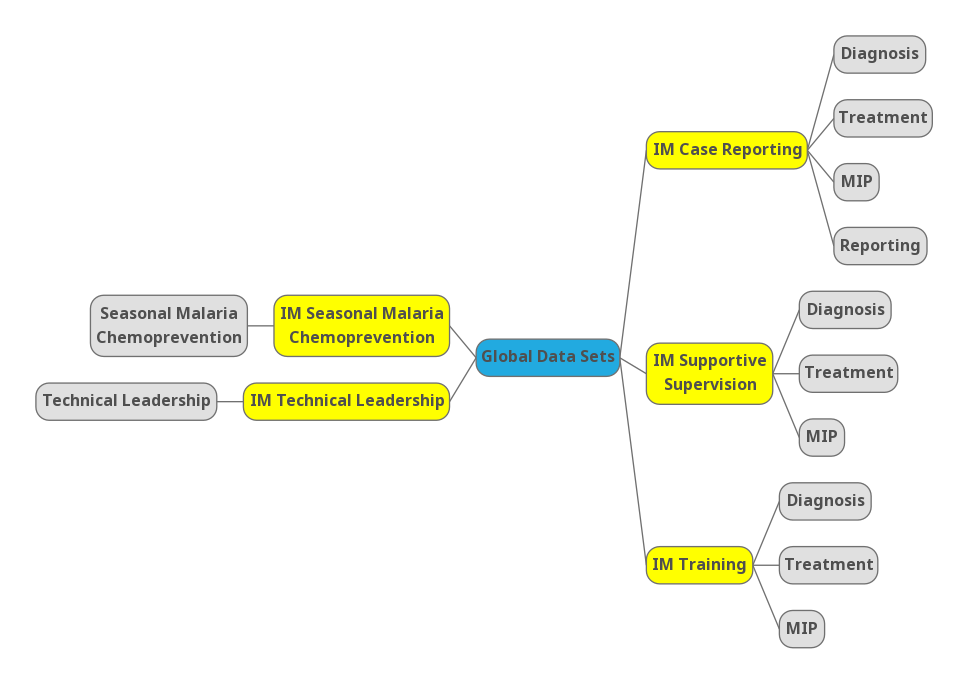
\includegraphics[width=13.47in]{./images/im datasets}

Global datasets are divided into sections (in grey) that groups IM data elements into multiple subheadings for ease of data collection.

There are five main sections:

\begin{enumerate}
\def\labelenumi{\arabic{enumi}.}
\tightlist
\item
  Diagnosis
\item
  Treatment
\item
  MIP
\item
  Technical leadership
\item
  Seasonal Malaria Chemoprevention
\end{enumerate}

We will talk about them in chapter 4.

\hypertarget{accessing-global-datasets.}{%
\subsubsection{Accessing Global Datasets.}\label{accessing-global-datasets.}}

\begin{enumerate}
\def\labelenumi{\arabic{enumi}.}
\tightlist
\item
  If you haven't already logged in yet, please log in now at:
\end{enumerate}

\href{https://im-dev.psi-mis.org/dhis-web-dataentry/index.action}{IM Data Hub demo}

\texttt{Username} :\textbf{\texttt{demoUser}} and \texttt{Password} : \textbf{\texttt{Temp1234!}}

\begin{enumerate}
\def\labelenumi{\arabic{enumi}.}
\setcounter{enumi}{1}
\tightlist
\item
  Search for the Data Entry App from Apps
\end{enumerate}

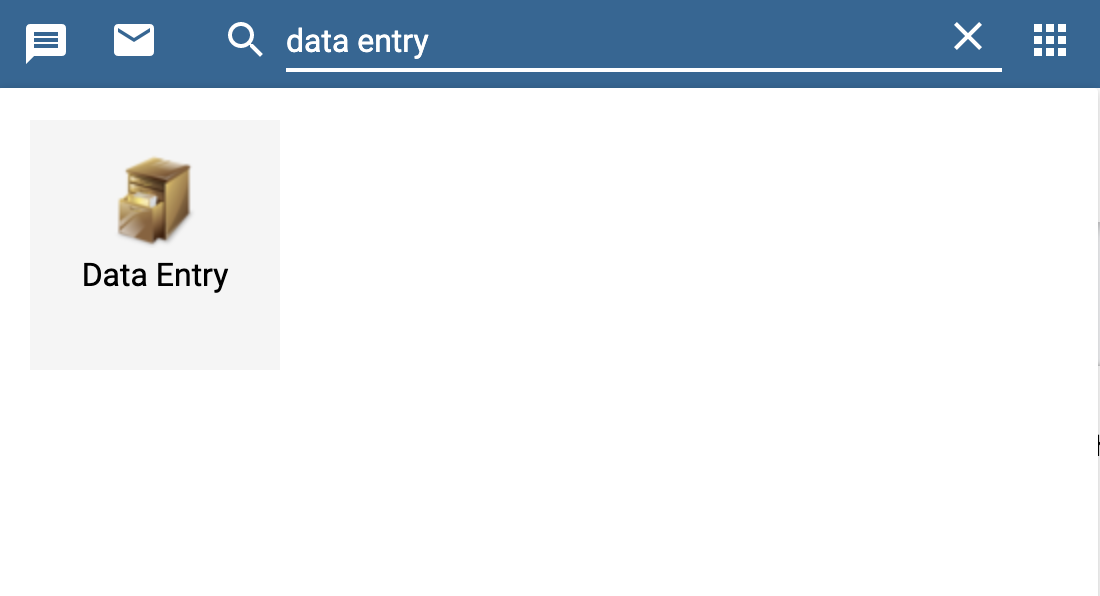
\includegraphics[width=15.28in]{./images/data-entry-app2}

\begin{enumerate}
\def\labelenumi{\arabic{enumi}.}
\setcounter{enumi}{2}
\item
  Click on the test world on top left if not already selected
\item
  Select \texttt{IM\ Case\ Reporting} data set and the period to report; this case October 2019.
\item
  Wait for the data entry form to load, and check that you can see the same screen as in Fig. 5 below. Congratulations! You can now start reporting..
\end{enumerate}

Before completing the records, please notice the \texttt{Run\ validation} button at the top right. We will talk about this in section 6.

The complete button submits the records into the data hub.

\hypertarget{country-specific-datasets}{%
\subsection{Country Specific Datasets}\label{country-specific-datasets}}

\hypertarget{impact-malaria-data-specification}{%
\chapter{Impact Malaria Data Specification}\label{impact-malaria-data-specification}}

\hypertarget{introduction-1}{%
\section{Introduction}\label{introduction-1}}

IM data is specified through the use indicators. Indicators consist of a numerator, denominator, and a count. The numerator and denominator are data elements, and the count specifies the applied operation. Counts can be a percentage, a number, or a ratio.

In this chapter, we are going to explore the IM indicators and how they are constructed in the Data Hub.

We'll start by a short introduction to data elements and how they form the base/source of the IM indicators. We'll then explore the different counts and wind up by showing you all the IM indicators.

\hypertarget{metadata-specification}{%
\chapter{Metadata Specification}\label{metadata-specification}}

\hypertarget{introduction-2}{%
\section{Introduction}\label{introduction-2}}

In the previous chapters, we learned about the IM \& PMP indicators and how they are stored and constructed in the Data Hub. That is essential knowledge for you to start monitoring IM indicator data from the source to how they are presented in the IM Data Hub.

In this chapter, we'll dive deep to the bottom and explore what lies underneath beneath the IM Data Hub, the metadata. Metadata is data about data. Interesting?

Let's get started!

\hypertarget{customization-troubleshooting-im-data-hub}{%
\chapter{Customization \& Troubleshooting IM Data Hub}\label{customization-troubleshooting-im-data-hub}}

\bibliography{book.bib,packages.bib}


\end{document}
